\documentclass[../main.tex]{subfiles}
\graphicspath{{\subfix{../img/}}}
\begin{document}

\newpage
\section{Lösungskonzept}



In diesem Kapitel wird das gewählte Lösungskonzept ''Simpel'' (siehe Anhang \ref{a3:loesungsvariante_Simpel}) näher erläutert. Wieso das Lösungskonzept ''Beweglich'' ausgeschieden ist, lese im Anhang \ref{a3:EntscheidLösungsvariante}. Bei dem gewählten Konzept liegt der Schwerpunkt auf einer möglichst einfachen Lösung, da ein einfach konstruiertes System in der Regel robuster im Einsatz ist. Im folgenden Text wird für jede Teilfunktion die einfachste Lösung erarbeitet und beschrieben.

\begin{figure}[H]
\centering
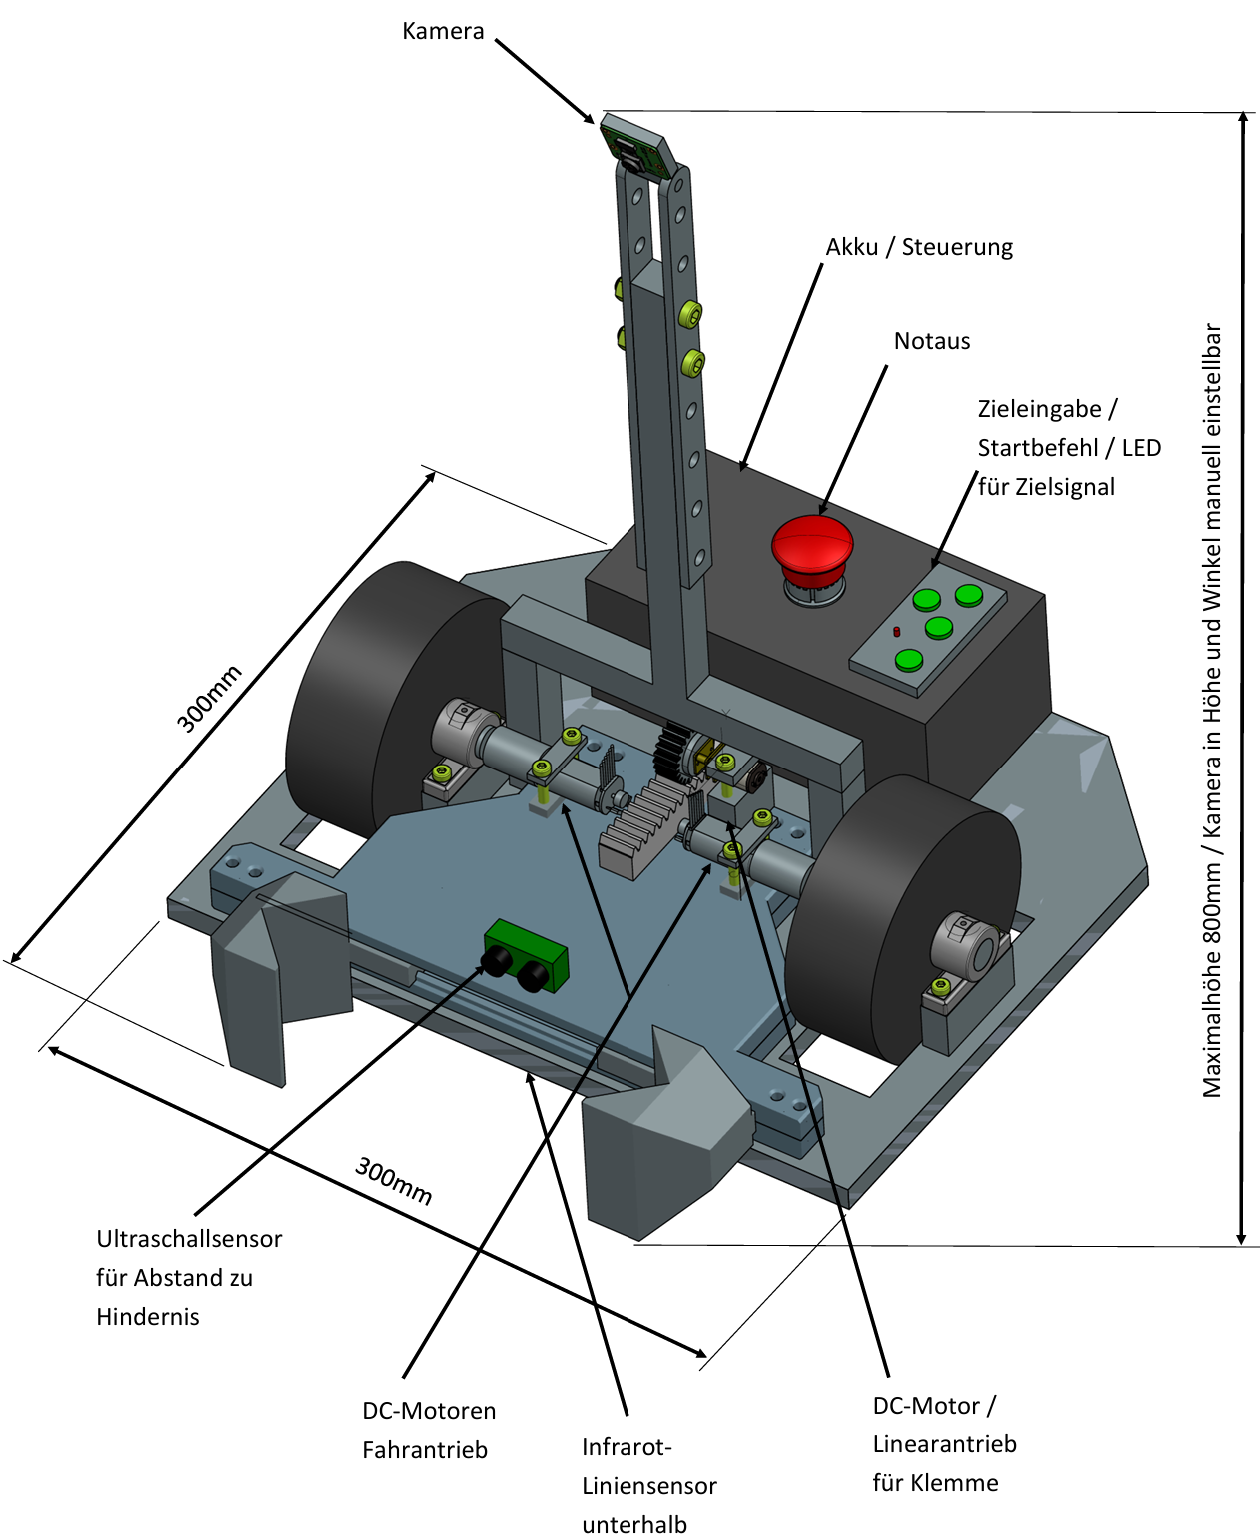
\includegraphics[width=0.85\linewidth]{Skizze Konzept beschriftet.png}
\caption{Konzept-Skizze Fahrzeug}
\label{img:Konzept-Skizze_Fahrzeug}
\end{figure}


\subsection{Ablauf}

Im Ablaufdiagramm (Abbildung \ref{img:ablaufdiagramm}) wird der Ablauf des Roboters von Start bis Ziel übersichtlich aufgezeigt.

\begin{figure}[H]
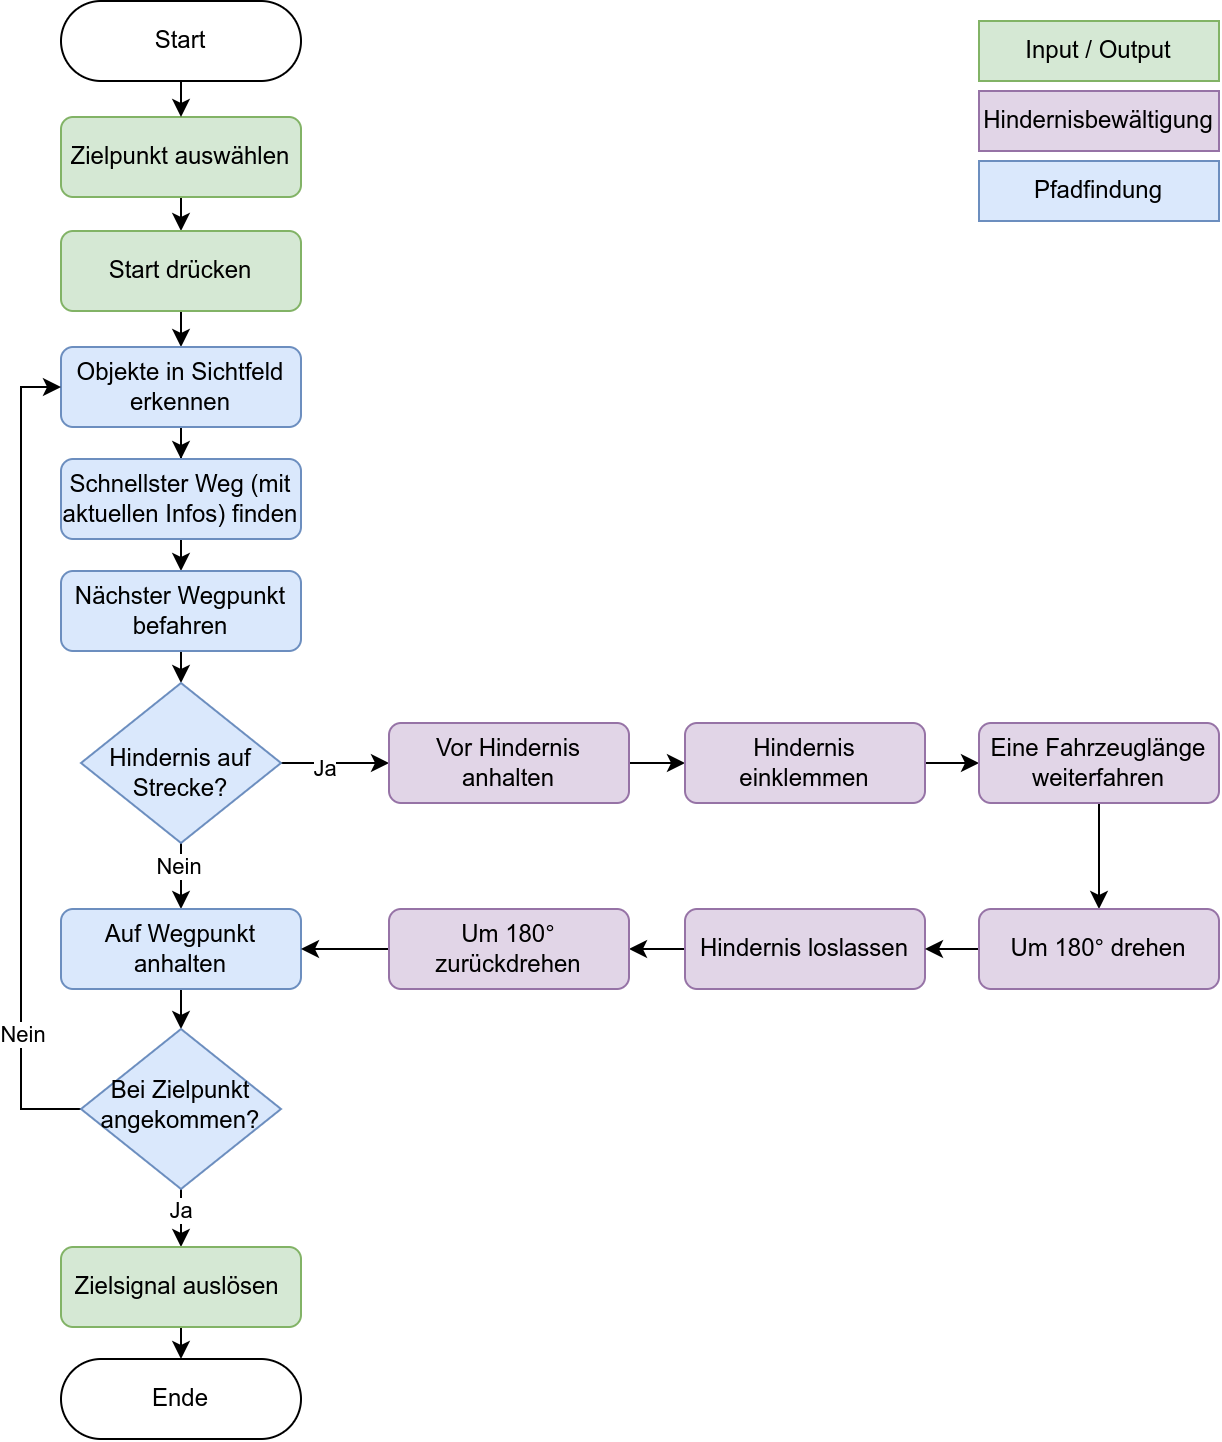
\includegraphics[width=0.9\textwidth]{img/lösungskonzpet/Ablaufdiagramm.png}
\caption{Ablaufdiagramm}
\label{img:ablaufdiagramm}
\end{figure}



\subsection{Wegfindung} %Objekterekennung, idealer Weg, 
Die Objekterkennung wird mithilfe eines Raspberry Pi und der dazugehörigen Pi-Kamera durchgeführt. Dabei werden Pylonen, Hindernisse und Wegpunkte erkannt. Als Software kommt YOLO zum Einsatz. Die erfassten Daten dienen anschliessend der Wegfindung, wobei versucht wird, den kürzest möglichen Weg ohne Pylonen zu ermitteln. Hierfür wird der Dijkstra-Algorithmus verwendet. Da anfangs wahrscheinlich nicht das gesamte Feld erfasst wird, wird jeweils der nächstbeste Punkt bestimmt und die Prozedur dort wiederholt.



\subsection{Fortbewegung} 

Die Fortbewegung wird nach dem Prinzip Roomba realisiert. Wie der Name schon erahnen lässt, handelt es sich dabei um ein ähnliches System, wie wir es von Staubsauger-Robotern kennen. Das Prinzip besteht aus zwei einzeln angetriebenen Rädern und einem Stützelement. Die angetriebenen Räder können unabhängig in beide Drehrichtungen angetrieben werden, wodurch ein Wenden an Ort und Stelle ermöglicht wird. Die beiden Räder sind in Längsrichtung zentrisch angeordnet, damit sich das Fahrzeug um den eigenen Mittelpunkt drehen kann, ohne dass ein Versatz entsteht. Weitere Details dazu befinden sich im Anhang unter \ref{a3:}

Als Antriebsmotoren werden Brushed-DC-Motoren verwendet, die über eine H-Brücke mit einem PWM-Signal angesteuert werden können. Jeder Motor verfügt über einen Encoder, der überwacht, dass beide Motoren die gleiche Anzahl an Umdrehungen ausführen. Gesteuert werden die Motoren von einem TinyK22, der die H-Brücke ansteuert. Weitere Details können im Anhang unter \ref{a3:Fahrantrieb} nachgeschlagen werden.

Der TinyK22 ist über eine UART-Schnittstelle mit dem Raspberry Pi verbunden (siehe Abbildung \ref{img:UART_Schnittstelle}). Zunächst sendet der TinyK22 das gewünschte Ziel an den Raspberry Pi. Anschliessend teilt der Raspberry Pi dem TinyK22 mit, um welchen Winkel das Fahrzeug ausgerichtet werden muss, um den nächsten Zielpunkt zu erreichen. Dreht sich das Fahrzeug auf die angepeilte Linie, erkennt dies der Liniensensor. Wird die Linie nicht erkannt, sucht das System diese durch Drehungen im Bereich von ±15 Grad. Sobald die Linie gefunden wird, meldet der TinyK22 dem Raspberry Pi, wie weit sich das Fahrzeug gedreht hat.
\begin{figure}[H]
\centering
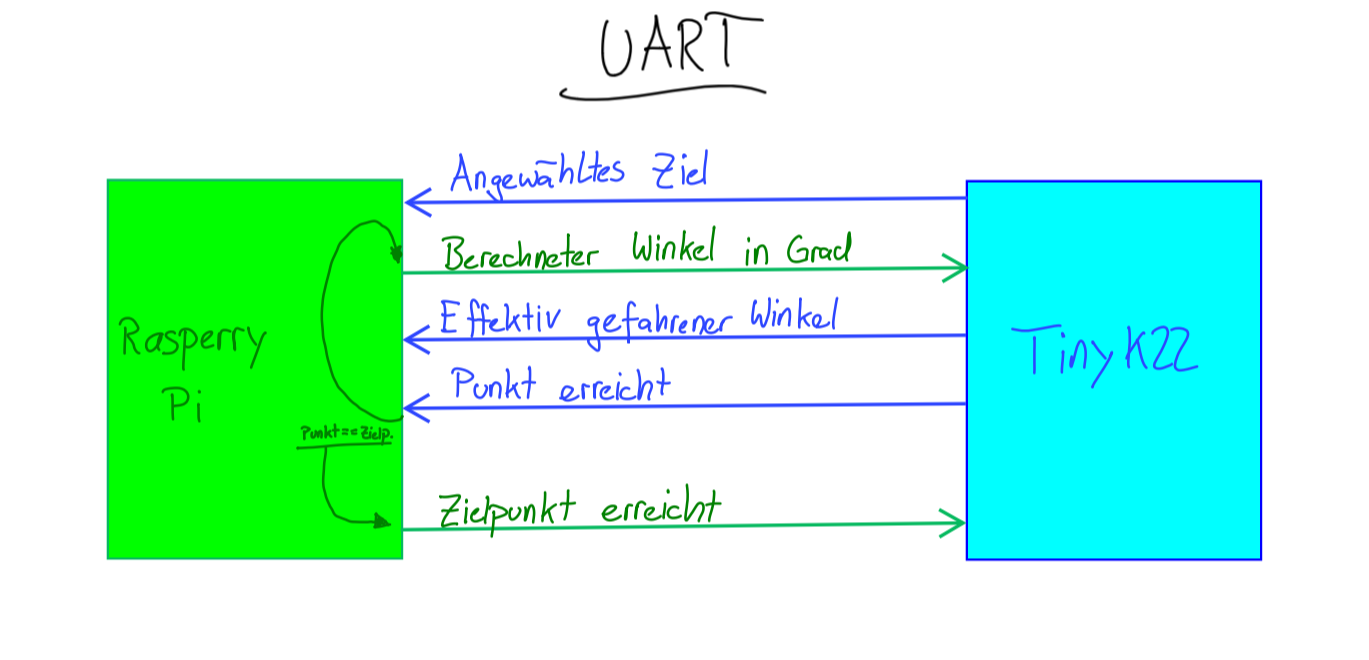
\includegraphics[width=0.7\textwidth]{img/lösungskonzpet/Skizzen/UART_Schnittstelle.png}
\caption{UART Schnittstelle}
\label{img:UART_Schnittstelle}
\end{figure}
Das Fahrzeug folgt der Linie mithilfe des Liniensensors. Erkennt der Sensor eine breitere Linie, also einen Punkt, informiert der TinyK22 den Raspberry Pi, stoppt das Fahrzeug, und der Vorgang beginnt erneut. Sobald das Fahrzeug den Zielpunkt erreicht, signalisiert der Raspberry Pi dies dem TinyK22, der daraufhin eine LED blinken lässt.
%Schnittstelle Raspy zurüfür Richtung, Antrieb, Mechanik, Zielsignal, Liniensensor, Anhalten




\subsection{Hindernisbewältigung} %Hindernisvermessung, Antrieb, Mechanik,
Erkennt der Ultraschallsensor ein Hindernis auf der Linie, wird dies kontinuierlich während der Fahrt überwacht. Sobald ein Hindernis in 30 cm Entfernung detektiert wird, verlangsamt sich das Fahrzeug und fährt langsam darauf zu, bis es zwischen den zwei Klemmbacken positioniert ist. Diese Distanz ist vorprogrammiert, und das Fahrzeug hält an. Danach wird der Schrittmotor angesteuert, der das Hindernis ergreift und mit einem Mechanismus anhebt.
Das Fahrzeug fährt anschliessend eine Fahrzeuglänge vor, wobei die Encodermessung die Distanz überwacht. Danach dreht es sich um 180 Grad, und der Schrittmotor löst die Klemmen. Das Fahrzeug fährt nun ein Stück zurück, um das Hindernis nicht mehr zwischen den Klemmbacken zu haben, und vollzieht eine weitere 180-Grad-Drehung. Abschliessend fährt das Fahrzeug mithilfe des Liniensensors entlang der Linie zum nächsten Punkt.
\begin{figure}[H]
\centering
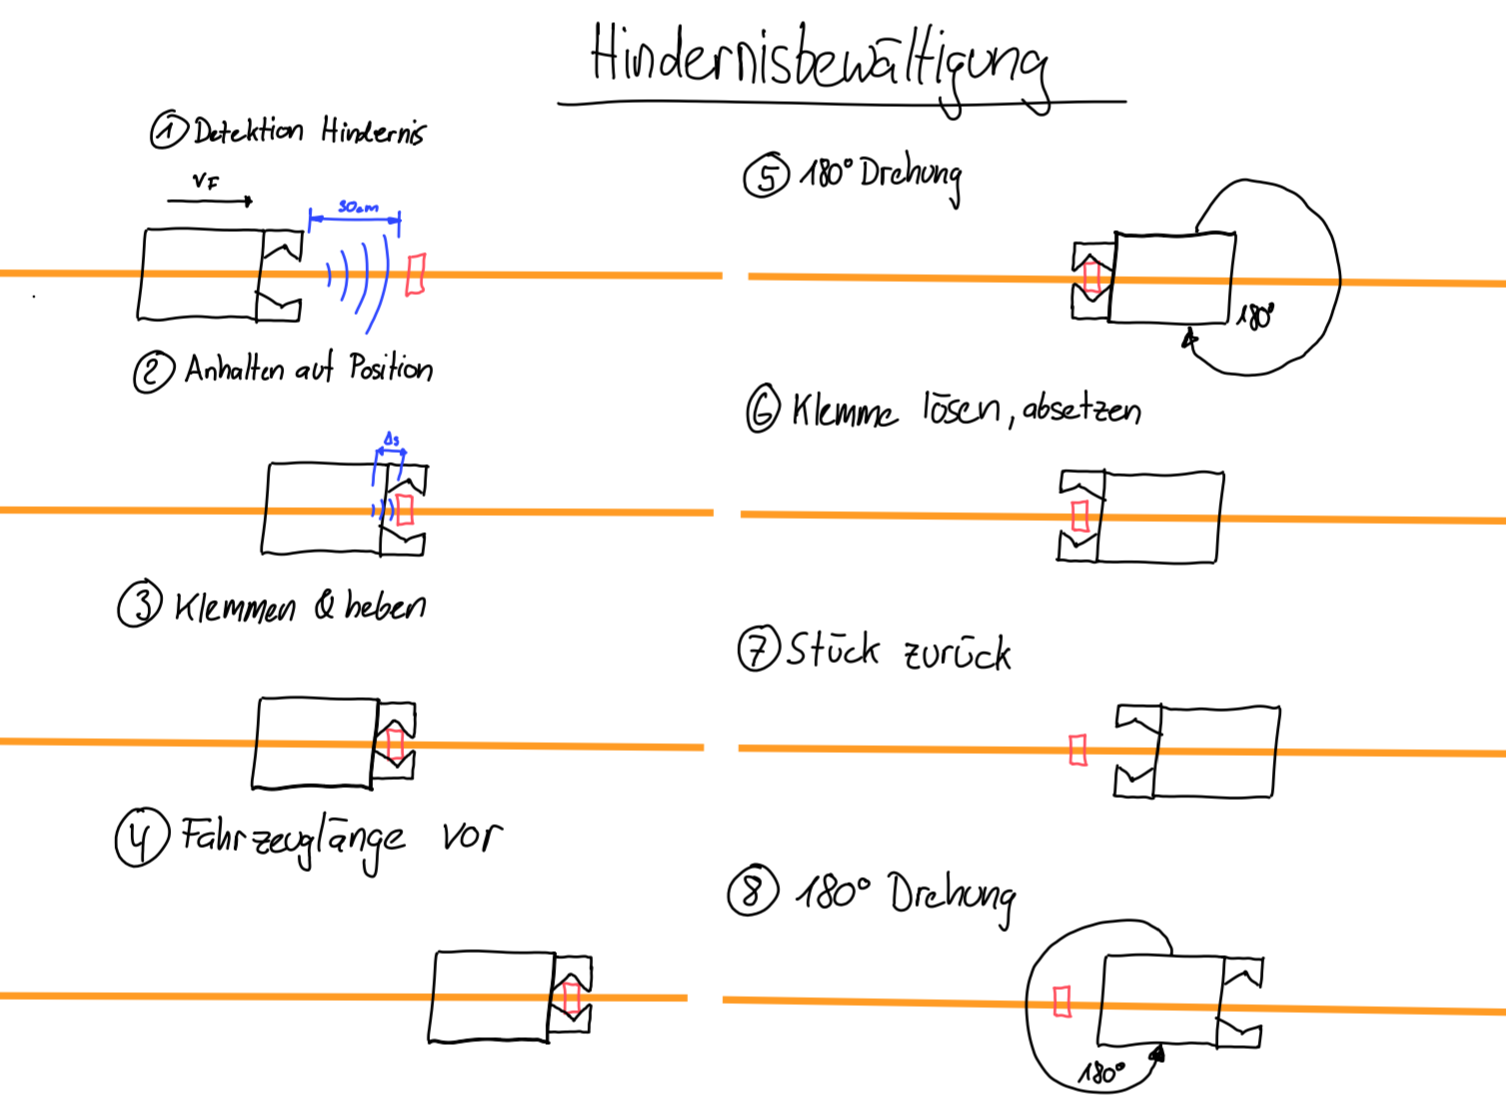
\includegraphics[width=0.8\textwidth]{img/lösungskonzpet/Skizzen/Skizze_Hindernisbewältigung.png}
\caption{Hindernisbewältigung}
\label{img:Skizze_Hindernisbewältigung}
\end{figure}



\subsection{Energiequelle}
Aus der Technologierecherche hat sich herausgestellt, dass der LiPo-Akku der am besten geeignete Akku im Vergleich zu Li-Ion- und NiMH-Akkus ist. Dies liegt insbesondere an seiner höheren Leistungsdichte, besseren Leistungsabgabe und der Flexibilität in der Formgebung. Weitere Details dazu können im Anhang unter  \ref{a3:Energiequelle} nachgelesen werden.




\subsection{Wegfindungssoftware}

Um den schnellsten Weg ins Ziel zu finden, wird der Graph in der Software abgespeichert
und der kürzeste Weg mittels Dijkstra Algorithmus berechnet. Sobald neue Informationen der Strecke erkannt werden, wird der Graph entsprechend angepasst und der kürzeste Weg wird anhand der aktuellen Position neu ermittelt.
Ursprünglich haben alle Linien im Graphen eine einheitliche Gewichtung. 

Je nach neu erhaltener Information werden andere Anpassungen am Graphen vorgenommen:
\begin{itemize}
    \item Pylon auf Wegpunkt erkannt: Wegpunkt (Knote) wird aus dem Graphen entfernt
    \item Linie wurde entfernt: Linie (Kante) wird aus dem Graphen entfernt.
    \item Hindernis auf Linie erkannt: Linie (Kante) erhält mehr Gewichtung.
\end{itemize}









% Beschreib von Aufbau
% Schnittstelle TiynK22 Raspy (Schnittstelle Bild)
% Problem Kap
% 








% Alter Teil===========================================================================================================================================================



\subsection{Hardware Steuerung}
Zur Auswahl stehen verschiedene Mikrocontroller, darunter der Arduino, der TinyK22 und der ESP32. Im Rahmen dieses Konzepts, das auf Einfachheit setzt, stellt der ESP32 jedoch eine überdimensionierte Lösung dar, da weder WiFi noch Bluetooth in unserem Anwendungsfall benötigt werden. Zudem hat der ESP32 einen höheren Stromverbrauch, der in diesem Kontext nicht gerechtfertigt ist. Aus diesen Gründen scheidet der ESP32 aus.

Der Vorteil des Arduinos liegt in seiner grossen Community und der umfangreichen Online-Hilfe, die zur Verfügung steht. Da jedoch die Elektrotechniker keine Programmiererfahrung in C++ haben und nicht jeder Arduino eine Debugging-Funktion bietet, ist der Arduino nicht die einfachste Lösung.

Der TinyK22 hingegen wurde im Modul Mc Fun ausführlich behandelt. Er bietet eine benutzerfreundliche Programmierumgebung mit integriertem Debugger und wird in C programmiert. Zudem können bei Fragen die Dozenten konsultiert werden, die bereits über umfangreiche Erfahrung mit dem TinyK22 verfügen. In unserem Anwendungsfall stellt der TinyK22 daher die einfachste und effektivste Lösung für die Programmierung dar.


\subsection{Objekterkennung Hindernis}
Das Hindernis wird bereits zu Beginn von der Kamera erkannt. Zur Distanzmessung des Hindernisses wird dann auf einen Ultraschallsensor gewechselt, da dieser ab 3 cm präzise Werte liefert. Zudem ist die Ansteuerung des Ultraschallsensors sehr einfach, da er nur über die Trigger- und Echo-Pins gesteuert wird. Der Time of Flight (TOF) Sensor hingegen wird über eine I2C-Schnittstelle ausgelesen. Im Kapitel Hardware-Test zeigt sich, dass die Messwerte beider Sensoren grundsätzlich ähnlich sind. Der TOF-Sensor hat jedoch den Nachteil von Messfehlern bei direkter Sonneneinstrahlung. Aus diesen Gründen fiel die Wahl auf den Ultraschallsensor.


\subsection{Objekterkennung Pylone}
Die Pylonen werden mit der Kamera erkannt, und zwar mithilfe von Objekterkennungssoftware. Obwohl die Kamera eine komplexere Lösung darstellt, kann der Ultraschallsensor aufgrund der angeschrägten Fläche keinen validen Messwert liefern, ebenso wie der TOF-Sensor. Daher ist die Kamera die zuverlässigste und effektivste Methode, um die Pylonen zu erkennen.


\subsection{Streckenerkennung}
Die Streckenerkennung setzt sich aus zwei Teilen zusammen. Zunächst muss an dem Punkt erkannt werden, in welche Richtung das Fahrzeug weiterfahren soll. Dies wird durch eine Kamera in Verbindung mit einem Raspberry Pi realisiert. Der Raspberry Pi analysiert das Bild und berechnet, um wie viel Grad sich das Fahrzeug drehen muss, um der gewünschten Richtung zu folgen.

Der zweite Teil der Streckenerkennung sorgt dafür, dass das Fahrzeug der Linie folgt. Dies wird durch einen Liniensensor aus Fototransistoren erreicht, der den Unterschied zwischen der Linie und dem Boden erkennen kann. Auf dieser Grundlage steuert der Sensor das Fahrzeug so, dass es konstant auf der Linie bleibt.

\subsubsection{Streckenerkennung Kamera}

TODO: Gian
- Wegpunkt wird mittels Objekterkennung erkannt (siehe ref)
- Linien bei Wegpunkt erkennen
  - Canny Edge Detection (Technologierecherche)
  - Hough Line Transform



\subsection{Objekterkennung Software}







\newpage
\subsection{Aufnahme Hindernis}
Wie bereits beschrieben wurde das Greifkonzept 'Klemme seitlich' ausgewählt (siehe \ref{loesungsvariante_Simpel}).
Damit dieses erfolgreich umgesetzt werden kann, wurden Dimensionen vom Greifer definiert  sowie ein passendes Konzept für den Mechanismus gefunden. Zusätzlich wurde der hebe Mechanismus und der Greifmechanismus so konstruiert das es mit einem Motor angesteuert werden kann.\\
Die Recherche und Entscheidungen die zu diesen ausgearbeiteten Konzept geführt hat sind im Anhang: \ref{hier muss noch ein Anhang hin} ersichtlich. Das Design, ersichtlich in Abbildung \ref{fig:greifarm_oben} und \ref{fig:greifarm_unten} besteht aus einer Kombination von Zahnrädern für die Klemmen sowie einer linearen Bewegung für das Anheben der ganzen Konstruktion mit Hindernis.

\begin{figure}[h!]
    \centering
    % Erste Minipage für das obere Bild
    \begin{minipage}[t]{0.45\textwidth}
        \centering
        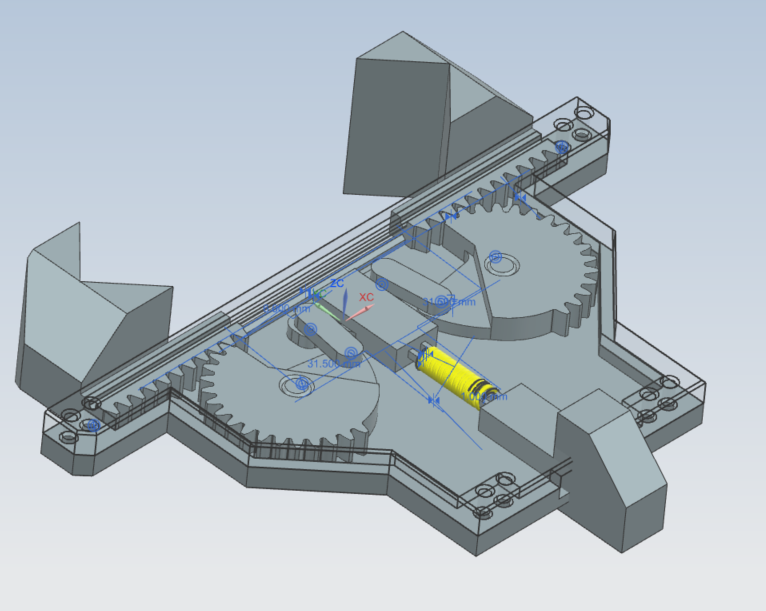
\includegraphics[width=\textwidth]{img/lösungskonzpet/hindernissaufnahme/Greifarm_oben.PNG}
        \caption{Greifarm oben}
        \label{fig:greifarm_oben}
    \end{minipage}
    \hfill
    % Zweite Minipage für das untere Bild
    \begin{minipage}[t]{0.45\textwidth}
        \centering
        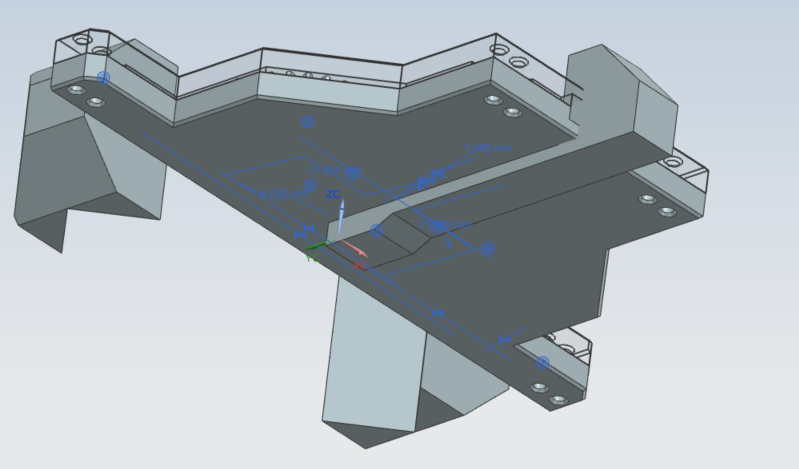
\includegraphics[width=\textwidth]{img/lösungskonzpet/hindernissaufnahme/Greifarm_unten.PNG}
        \caption{Greifarm unten}
        \label{fig:greifarm_unten}
    \end{minipage}
\end{figure}

%Im anhang sollte das stehehen
%allgemeines Konzept, etc entscheidung aus konzeptfindung
%Entscheidung alles mit einem Motor

\subsubsection{Funktionalitäten}
Wie bereits im Kapitel \ref{} beschrieben soll das Konzept folgende Anforderungen mit einem Motor erfüllen.
\begin{enumerate}
    \item Greifen
    \item Anheben
    \item Senken
    \item Loslassen
\end{enumerate}

Zusätzlich soll die Konstruktion helfen, Fehler bei der Messung auszukorrigieren.
\begin{enumerate}
    \item Korrektur Winkel (bis zu 15°, siehe Kapitel \ref{loes:winkel_verschiebung})
    \item Korrektur Distanz (bis zur Hälfte $b$, was 2.25 cm ist, siehe Kapitel \ref{loes:winkel_verschiebung})
    \item Korrektur Offset (bis zu 2 cm, siehe Kapitel \ref{loes:abstand_klemmen})
\end{enumerate}


\subsubsection{Dimensionen Greifarm}
Wie bereits im Kapitel \ref{a3:Präzision} erwähnt, ist die Präzision, die mechanisch gewonnen werden kann, sehr relevant für dieses Konzept. Damit dies auch funktioniert, wurden die passenden Dimensionen der Klemme eruiert. 

\paragraph{Winkel Verschiebung} \label{loes:winkel_verschiebung}
Nach Aufgabenstellung kann das Hindernis bis zu 15° verschoben sein.
In der Abbildung \ref{img:loes_winkel_hinderniss} ist dies bildlich dargestellt.

\begin{figure}[H]
        \centering
        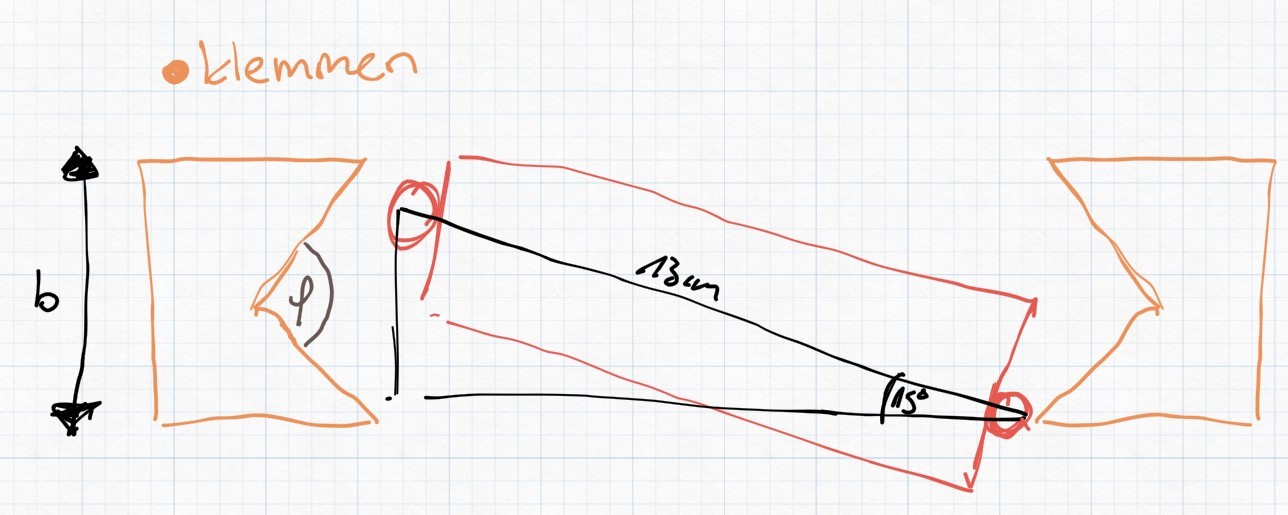
\includegraphics[width=0.48\textwidth]{img/lösungskonzpet/hindernissaufnahme/winkekl_klemmen.jpg}
        \caption {Möglicher Winkel des Hinderniss}
        \label{img:loes_winkel_hinderniss}
\end{figure}

Damit kann $b$ ausgerechnet werden:

\[
b = 13cm * sin(15) = 3.36cm
\]

Für genügend Sicherheit wurde entschieden das $b = 4.5cm$ ist. Diese Sicherheit hilft ebenfalls Fehler in der Distanzmessung auszugleichen.

$\varphi$ wurde 90° gewählt, dies war eine Annahme und wurde im Kapitel \ref{} getestet.

\newpage
\paragraph{Abstand der Klemmen} \label{loes:abstand_klemmen}
Der Abstand der Klemmen wurde anhand der Aufgabenstellung eruiert und ist in Abbildung \ref{img:loes_abstand_klemmen} ersichtlich. Das Hindernis kann 2 cm von der Linie entfernt sein. Das heisst das Maximale Offset ist 2 cm (In Abbildung Orange). Zusätzlich kommt die Winkel Reserve, die Distanz wurde im Kapitel \ref{loes:winkel_verschiebung} eruiert (In der Abbildung Blau). Ebenfalls in der Abbildung enthalten sind Reserve für Fehlmessungen (Rot), Reserve Festigkeit, die für nötig ist, um die Druckkräfte auszuhalten (Violett) und die Hälfte des Hindernis (Gelb)

\begin{figure}[H]
        \centering
        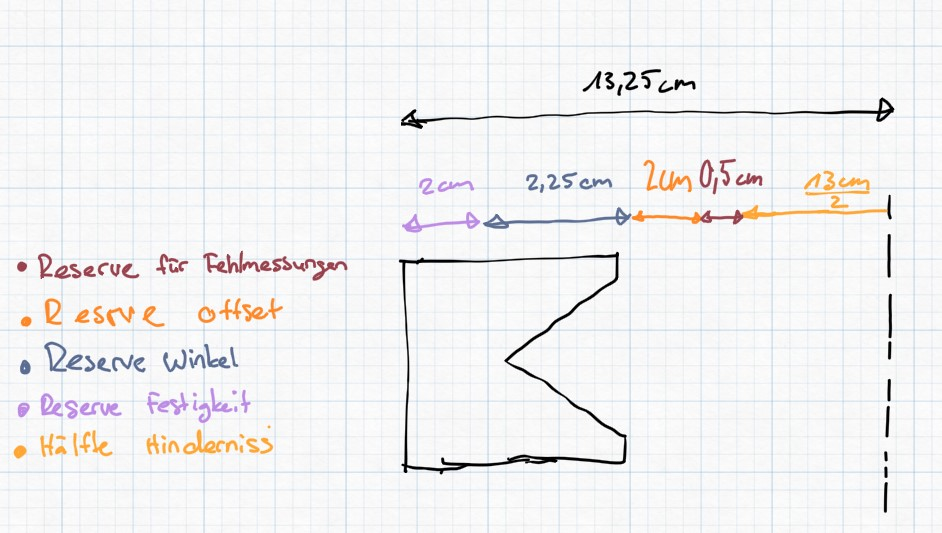
\includegraphics[width=0.48\textwidth]{img/lösungskonzpet/hindernissaufnahme/dimensionen_klemme.jpg}
        \caption {Abstand zwischen den Klemmen}
        \label{img:loes_abstand_klemmen}
\end{figure}

\newpage


\subsection{Rotation / Translation Hindernis}





\end{document}